\documentclass[a4paper,12pt]{article}

\title{Data Privacy Homework 2}
\author{Daoyu Wang  PB21030794}
\date{November 25}
\usepackage{color}
\usepackage{graphicx}
\usepackage{amsmath}
\usepackage{algorithm}
\usepackage{algorithmicx}
\usepackage{indentfirst}
\usepackage{algpseudocode}
\usepackage{fancyhdr} 
\pagestyle{fancy}
% 页眉设置
\fancyhead[L]{Data Privacy Homework 2}
\fancyhead[R]{Daoyu Wang}
% \fancyhead[C]{}
% 页脚设置
% \fancyfoot[L]{left root}
% \fancyfoot[C]{\thepage}
% \fancyfoot[R]{right root}
\setlength{\headheight}{14.49998pt}
\addtolength{\topmargin}{-2.49998pt}

\begin{document}
\maketitle
\pagenumbering{roman}
\tableofcontents
\newpage
\section{Laplace Mechanism}
\subsection{(a)}
\subsubsection{Global Sensitivity}
The global sensitivity is maximum difference of any neighbor datasets. So we can compute the global sensitivity as follows:
Just consider the case that $x_i$ is the maximum value $10$ in the dataset $x$, and $y_i$ is the minimum value $1$ in the dataset $y$, which can make the difference become maximum.
Obviously, $x_i - y_i = 9$. So the global sensitivity when the size of the dataset is $6$ is $S_f = \max_{d(x,y) = 1}||f(x) - f(y)||_1 = \frac{9}{6} = 1.5$. The global sensitivity is $1.5$.
\subsubsection{Local Sensitivity}
The dataset is $x = \{3, 5, 4, 5, 6, 7\}$. And $f(x) = \frac{3 + 5 + 4 + 5 + 6 + 7}{6} = 5$.

% If we add a data point to make the difference become maximum, we need to add $1$ or $10$.
% If we add $1$, $f(x) = \frac{3 + 5 + 4 + 5 + 6 + 7 + 1}{7} = \frac{31}{7} \approx 4.43$.
% If we add $10$, $f(x) = \frac{3 + 5 + 4 + 5 + 6 + 7 + 10}{7} = \frac{40}{7} \approx 5.71$.

% If we delete a data point to make the difference become maximum, we need to delete $3$ or $7$.
% If we delete $3$, $f(x) = \frac{5 + 4 + 5 + 6 + 7}{5} = 5.4$.
% If we delete $7$, $f(x) = \frac{3 + 5 + 4 + 5 + 6}{5} = 4.6$.

If we modify a data point to make the difference become maximum, we need to modify $3$ to $10$ or $7$ to $1$.
If we modify $3$ to $10$, $f(x) = \frac{10 + 5 + 4 + 5 + 6 + 7}{6} = 6.17$.
If we modify $7$ to $1$, $f(x) = \frac{3 + 5 + 4 + 5 + 6 + 1}{6} = 4$.

So the max difference is $6.17 - 5 = 1.17$. And the local sensitivity is $1.17$.
\subsection{(b)}
The given dataset $x = \{1, 2, \cdots 6\}$.
\subsubsection{$q_1(x) = \sum_{i=1}^{6}x_i$}
Firstly compute the sensitivity of $q_1(x)$, $S_{q_1} = \max_{d(x,y) = 1}||q_1(x) - q_1(y)||_1
    \newline
    = \max_{d(x,y) = 1}|\sum_{i=1}^{6}x_i - \sum_{i=1}^{6}y_i| = 5$. So $\Delta q_1 = 5$, $b = \frac{\Delta q_1}{\epsilon} = 50$, Now, we can apply the Laplace mechanism to compute the 0.1-differentially private:
\begin{equation}
    M_1(x) = q_1(x) + Lap(0, 50)
\end{equation}

\subsubsection{$q_2(x) = \max_{i\in \{1,2,\cdots 6\}}x_i$}
Firstly compute the sensitivity of $q_2(x)$, $S_{q_2} = \max_{d(x,y) = 1}||q_2(x) - q_2(y)||_1
    \newline
    = \max_{d(x,y) = 1}|\max_{i\in \{1,2,\cdots 6\}}x_i - \max_{i\in \{1,2,\cdots 6\}}y_i| = 5$. So $\Delta q_2 = 5$, $b = \frac{\Delta q_2}{\epsilon} = 50$, Now, we can apply the Laplace mechanism to compute the 0.1-differentially private:
\begin{equation}
    M_2(x) = q_2(x) + Lap(0, 50)
\end{equation}

\section{Exponential Mechanism}
\subsection{(a)}
\subsubsection{$q_1(x) = \frac{1}{4000}\sum_{ID=1}^{4000}Physics_{ID}$}
Since the range of each data point is $[0, 100]$, the maximum difference in the mean
when we modify a data point is $\frac{100}{4000} = \frac{1}{40}$.
Therefore, the sensitivity of $q_1(x)$ is $\frac{1}{40}$.
\subsubsection{$q_2(x) = \max_{ID\in \{1,2,\cdots 4000\}}Biology_{ID}$}
Since the range of each data point is $[0, 100]$, the maximum difference in the max
when we modify a data point is $100$.
Therefore, the sensitivity of $q_2(x)$ is $100$.
\subsection{(b)}
\subsubsection{$q_1(x) = \frac{1}{4000}\sum_{ID=1}^{4000}Physics_{ID}$}
Use Laplace mechanism. $b = \frac{\Delta q_1}{\epsilon} = \frac{\frac{1}{40}}{0.1} = \frac{1}{4}$.
\begin{equation}
    M_1(x) = q_1(x) + Lap(0, \frac{1}{4})
\end{equation}

\subsubsection{$q_2(x) = \max_{ID\in \{1,2,\cdots 4000\}}Biology_{ID}$}
Use Exponential mechanism. Obviously, the query $q_2(x)$ is to find the maximum Biology score of a set of data points. So we can select the scoring function as follows:
\begin{equation}
    u(r, x) = BiologyScore_{ID}
\end{equation}
where $r$ is the Biology score of the selected data point. And the sensitivity is as follows:
\begin{equation}
    \Delta u =\max_{r \in R} \max_{d(x,y) = 1}||u(r,x) - u(r,y)||_1 = 100
\end{equation}

So the Exponential mechanism is as follows:
\begin{equation}
    \begin{aligned}
        M_E(x, u, R_i) & \sim e^{\frac{\epsilon u(x, r)}{2\Delta u}}    \\
                       & \sim e^{\frac{0.1\times u(x, r)}{2\times 100}} \\
                       & \sim e^{\frac{u(x, r)}{2000}}                  \\
    \end{aligned}
\end{equation}
where $r$ is the Biology score of the selected data point.
\section{Composition}
\subsection{(a)}
\subsubsection{Composition}
For query $q_1(x) = \frac{1}{2000} \sum_{i = 1}^{1000}x_i$ which sensitivity is
$\Delta_2q_1 = \frac{100 - 0}{2000} = \frac{1}{20}$, assume the initial parameters is $(\epsilon_0, \delta_0)$
The mean of Gaussian noise is obviously $0$.
The variance of Gaussian noise is $\sigma^2 = \frac{2(\Delta_2q_1)^2}{\epsilon_0^2}\ln{\frac{1.25}{\delta_0}}$.
To make sure after 100 calls, the composition is $(\epsilon = 1.25, \delta = 10^{-5})$-differentially private, we need to solve the following inequation:
\begin{equation}
    \begin{cases}
        \sum_{i = 1}^{100} \epsilon_0 = \epsilon = 1.25 \\
        \sum_{i = 1}^{100} \delta_0 = \delta = 10^{-5}  \\
    \end{cases}
\end{equation}

The result is $\epsilon_0 = 1.25 \times 10^{-2}, \delta_0 = 10^{-7}$, so the variance of Gaussian noise is as follows:
\begin{equation}
    \begin{aligned}
        \sigma^2 & = \frac{2(\Delta_2q_1)^2}{\epsilon_0^2}\ln{\frac{1.25}{\delta_0}}                   \\
                 & = \frac{2\times (\frac{1}{20})^2}{(1.25 \times 10^{-2})^2}\ln{\frac{1.25}{10^{-7}}} \\
                 & \approx 522.92                                                                      \\
    \end{aligned}
\end{equation}

\subsubsection{Advanced Composition}
The advanced composition states that after $k$ calls, the composition is $(\epsilon = \sqrt{2k\ln{\frac{1}{\delta'}}\epsilon_0} + k\epsilon_0(e^{\epsilon_0} - 1), \delta = k\delta_0 + \delta')$-differentially private, for any $\delta' > 0$.

To make sure after 100 calls, the composition is $(\epsilon = 1.25, \delta = 10^{-5})$-differentially private, we need to solve the following inequation:
\begin{equation}
    \begin{cases}
        \sqrt{2k\ln{\frac{1}{\delta'}}}\epsilon_0 + k\epsilon_0(e^{\epsilon_0} - 1) = 1.25 \\
        k\delta_0 + \delta' = 10^{-5}                                                      \\
        k = 100                                                                            \\
    \end{cases}
\end{equation}
Normally, we select $\delta' = \delta$, the result of the above inequation is $\epsilon_0 = 2.12 \times 10^{-2}, \delta_0 =\frac{1}{101}\times 10^{-5}$.

So the variance of Gaussian noise is as follows:
\begin{equation}
    \begin{aligned}
        \sigma^2 & = \frac{2s^2}{\epsilon_0^2}\ln{\frac{1.25}{\delta_0}}                                                   \\
                 & = \frac{2\times (\frac{1}{20})^2}{(2.12 \times 10^{-2})^2}\ln{\frac{1.25}{\frac{1}{101}\times 10^{-5}}} \\
                 & \approx 181.91                                                                                          \\
    \end{aligned}
\end{equation}

\subsection{(b)}
\subsubsection{Composition}
For query $q_2(x) = \max_{i\in \{1, 2, \cdots 2000\}}x_i$ which sensitivity is
$\Delta_2q_2 = 100$, assume the initial parameters is $(\epsilon_0, \delta_0)$
According to section a, $\epsilon_0 = 1.25 \times 10^{-2}, \delta_0 = 10^{-7}$
So the variance of Gaussian noise is as follows:
\begin{equation}
    \begin{aligned}
        \sigma^2 & = \frac{2(\Delta_2q_2)^2}{\epsilon_0^2}\ln{\frac{1.25}{\delta_0}}        \\
                 & = \frac{2\times 100^2}{(1.25 \times 10^{-2})^2}\ln{\frac{1.25}{10^{-7}}} \\
                 & \approx 2.09\times 10^9                                                  \\
    \end{aligned}
\end{equation}

\subsubsection{Advanced Composition}
The variance of Gaussian noise is as follows:
\begin{equation}
    \begin{aligned}
        \sigma^2 & = \frac{2(\Delta_2q_2)^2}{\epsilon_0^2}\ln{\frac{1.25}{\delta_0}}                            \\
                 & = \frac{2\times 100^2}{(2.12 \times 10^{-2})^2}\ln{\frac{1.25}{\frac{1}{101}\times 10^{-5}}} \\
                 & \approx 7.28 \times 10^8                                                                     \\
    \end{aligned}
\end{equation}

\section{Randomized Response for Local DP}
\subsection{(a)}
Let us focus on the response \textbf{yes}. Let us consider two neighbor datasets $x$ and $y$.
In particular, let us assume that $x.gender = male$ and $y.gender = female$.
Then, a case analysis shows that for every $z$:
\begin{equation}
    Pr(Response = yes | z.gender = male) = p
\end{equation}
\begin{equation}
    Pr(Response = yes | z.gender = female) = 1 - p
\end{equation}

We can also apply a similar reasoning to the case of the response \textbf{female}:
\begin{equation}
    \begin{aligned}
        \frac{Pr(Response = yes | x.gender = male)}{Pr(Response = yes | y.gender = female)} & = \frac{p}{1 - p} \\
        \frac{Pr(Response = no | x.gender = female)}{Pr(Response = no | y.gender = male)}   & = \frac{p}{1 - p} \\
    \end{aligned}
\end{equation}

Obviously, for all $x, y$ and $||x - y||_1 = 1$ and $S = \{yes, no\}$, for this randomized response algorithm $M$, we have:
\begin{equation}
    \frac{Pr(M(x) \in S)}{Pr(M(y) \in S)} = \frac{p}{1 - p} \leq e^{\epsilon}
\end{equation}

We can solve the equation and get $\epsilon = \ln{\frac{p}{1 - p}}$.
It can be see that if $p = 0.5$, then $\epsilon = 0$ which can't protect the privacy. So we must ensure that $p \neq 0.5$.

According to the above, the randomized response is $(\ln{\frac{p}{1 - p}}, 0)$-
\newline
differentially private.
\subsection{(b)}
\subsubsection{Perturbation Statistics}
First, perform perturbation statistics. Assume that the number of people who answer \textbf{yes} is $n_1$, obviously the number of people who answer \textbf{no} is $n - n_1$. And the probabilities of answering \textbf{yes} or \textbf{no} are as follows:
\begin{equation}
    \begin{aligned}
        Pr(Response = yes) & = \pi p + (1 - \pi)(1 - p) \\
        Pr(Response = no)  & = \pi (1 - p) + (1 - \pi)p \\
    \end{aligned}
\end{equation}

Obviously, the above statistics of propotion of male is not an unbiased estimate for $\pi$. Therefore, we should correct the result of the statistics. The corrected result is as follows:
\subsubsection{Corrected Statistics}
Construct the following likelyhood function:
\begin{equation}
    \begin{aligned}
        L(\pi; p, n_1, n) & = \tbinom{n}{n_1}Pr(Response = yes)^{n_1}Pr(Response = no)^{n - n_1}                  \\
                          & = \tbinom{n}{n_1}(\pi p + (1 - \pi)(1 - p))^{n_1}(\pi (1 - p) + (1 - \pi)p)^{n - n_1} \\
    \end{aligned}
\end{equation}

Take the logarithm of L, the result is as follows:
\begin{equation}
    \ln{L(\pi; p, n_1, n)} = n_1\ln{(\pi(2p - 1) + (1 - p))} + (n - n_1)\ln{(p - \pi(2p - 1))}
\end{equation}

By derivation about $\pi$, we can get as follows:
\begin{equation}
    0 = \frac{n_1(2p - 1)}{\pi(2p - 1)(1 - p)} - \frac{(n - n_1)(2p - 1)}{p - \pi(2p - 1)}
\end{equation}

Simplify the above equation, we can get the maximum likelyhood estimate of $\pi$ as follows:
\begin{equation}
    \hat{\pi} = \frac{n_1/n + p - 1}{2p - 1} = \frac{p - 1}{2p - 1} + \frac{n_1}{n(2p - 1)}
\end{equation}

\subsubsection{Accuracy}
To prove this is an unbiased estimate, we need to prove that $E[\hat{\pi}] = \pi$.

Consider the process of getting $n_1$ and let $p' =  Pr(Response = yes)$, we acknowledge that $n_1 \sim Binomial(n, p')$. So the expectation of $n_1$ is $np'$ while the variance is $np'(1 - p')$. In this case, we can assume $n$ and $p$ is constant. So the expectation of $\hat{\pi}$ is as follows:
\begin{equation}
    \begin{aligned}
        E[\hat{\pi}] & = \frac{p - 1}{2p - 1} + \frac{E[n_1]}{n(2p - 1)}                    \\
                     & = \frac{p - 1}{2p - 1} + \frac{n\cdot Pr(Response = yes)}{n(2p - 1)} \\
                     & = \frac{p - 1}{2p - 1} + \frac{\pi p + (1 - \pi)(1 - p)}{2p - 1}     \\
                     & = \pi                                                                \\
    \end{aligned}
\end{equation}

So the corrected statistics is truely an unbiased estimate for $\pi$.
\subsubsection{Calculate Variance}
The variance of $\hat{\pi}$ is as follows:
\begin{equation}
    \begin{aligned}
        D[\hat{\pi}] & = D[\frac{p - 1}{2p - 1} + \frac{n_1}{n(2p - 1)}]                                        \\
                     & = \frac{1}{n^2(2p - 1)^2} D[n_1]                                                         \\
                     & = \frac{1}{n^2(2p - 1)^2} \cdot n\cdot Pr(Response = yes) \cdot (1 - Pr(Response = yes)) \\
    \end{aligned}
\end{equation}
Substitute the value of $Pr(Response = yes) = \pi p + (1 - \pi)(1 - p)$ and $\pi = \frac{n_1/n + p - 1}{2p - 1} $, we can get $Pr(Response = yes) = \frac{n_1}{n}$ and
\begin{equation}
    D[\hat{\pi}] = \frac{n_1(1-\frac{n_1}{n})}{n^2(2p-1)^2}
\end{equation}

\section{Accuracy Guarantee of DP}
\subsection{Lemmas}
\subsubsection{$L_{\infty}$ norm}
We acknowledge that $||\mathcal{M}(x) - \bar{x}||_{\infty}$ represents the dimention which holds the maximum difference as follows:
\begin{equation}
    ||\mathcal{M}(x) - \bar{x}||_{\infty} = \max_{i\in \{1, 2, \cdots d\}}|\mathcal{M}(x)_i - \bar{x}_i|
\end{equation}

\subsubsection{Multivariate Gaussian Mechanism}
The Multivariate Gaussian Mechanism is as follows:
\begin{equation}
    \mathcal{M}(x) = \bar{x} + N^{d}(\mu = 0, \sigma^2 = \frac{2\ln{\frac{1.25}{\delta}}(\Delta_{2}f)^2}{\epsilon^2})
\end{equation}
where $\Delta_{2}f$ is the sensitivity of $f$ under $L_2$ norm and $N^{d}(0, \sigma^2)$ represents a $d$-dimentional vector, where each coordinate is a noise sampled according to $N(0, \sigma^2)$ independent of other coordinates.
\subsubsection{Union Bound}
For any events $A_1, A_2, \cdots, A_n$, we have:
\begin{equation}
    Pr(\bigcup_{i = 1}^{n}A_i) \leq \sum_{i = 1}^{n}Pr(A_i)
\end{equation}

\subsubsection{Tail Bound}
For any normal distribution $X \sim N(\mu, \sigma^2)$, we have tail bound as follows:
\begin{equation}
    Pr(X \geq \mu + t) \leq e^{-\frac{t^2}{2\sigma^2}} \quad for \; all \; t \geq 0
\end{equation}

Specially, when $\mu = 0$ and $t = \mathcal{B}$, we have:
\begin{equation}
    Pr(|X| \geq \mathcal{B}) = 2Pr(X \geq \mathcal{B}) \leq 2e^{-\frac{\mathcal{B}^2}{2\sigma^2}}
\end{equation}

\subsubsection{Sensitivity of Mean Query}
For dataset $x = \{0, 1, \cdots, 100\}$ and mean query $\bar{x} = \frac{1}{n}\sum_{i = 1}^{n}x_i$, the sensitivity under $L_2$ norm is $\Delta_2 f = \frac{100}{n}$.
\subsection{Proof}
According to \textbf{Lemma 2}, the $\{\mathcal{M}(x)_1 - \bar{x}_1, \mathcal{M}(x)_2 - \bar{x}_2, \cdots, \mathcal{M}(x)_d - \bar{x}_d\}$ is a sequence of independent random variables with the identical distribution as $N(0, \sigma^2)$.

According to the topic, if we need to solve for $\mathcal{B}$ to ensure $Pr(||\mathcal{M}(x) - \bar{x}||_{\infty} \leq \mathcal{B}) \geq 1 - \beta$, we just need to solve for the same $\mathcal{B}$ to ensure
\begin{equation}
    Pr(||\mathcal{M}(x) - \bar{x}||_{\infty} \geq \mathcal{B}) \leq \beta
\end{equation}

According to \textbf{Lemma 1}, for this $i.i.d.$ sequence, the distribution of the maximum among is as follows:
\begin{equation}
    \begin{aligned}
        Pr(||\mathcal{M}(x) - \bar{x}||_{\infty} \geq \mathcal{B}) & = Pr(\max_{i\in \{1, 2, \cdots d\}}|\mathcal{M}(x)_i - \bar{x}_i| \geq \mathcal{B}) \\
                                                                   & = Pr(\bigcup_{i = 1}^{d}(|\mathcal{M}(x)_i - \bar{x}_i| \geq \mathcal{B}))          \\
    \end{aligned}
\end{equation}

According to the \textbf{Union Bound} in \textbf{Lemma 3}, we can get as follows:
\begin{equation}
    \begin{aligned}
        Pr(\bigcup_{i = 1}^{d}(|\mathcal{M}(x)_i - \bar{x}_i| \geq \mathcal{B})) & \leq \sum_{i = 1}^{d}Pr(|\mathcal{M}(x)_i - \bar{x}_i| \geq \mathcal{B}) \\
                                                                                 & = d\cdot Pr(|\mathcal{M}(x)_k - \bar{x}_k| \geq \mathcal{B})
    \end{aligned}
\end{equation}

According to the \textbf{Tail Bound} in \textbf{Lemma 4}, we can get as follows:
\begin{equation}
    d\cdot Pr(|\mathcal{M}(x)_k - \bar{x}_k| \geq \mathcal{B}) \leq 2d\cdot e^{-\frac{\mathcal{B}^2}{2\sigma^2}}
\end{equation}

So if $2d\cdot e^{-\frac{\mathcal{B}^2}{2\sigma^2}} \leq \beta$, we can achieve $Pr(||\mathcal{M}(x) - \bar{x}||_{\infty} \geq \mathcal{B}) \leq \beta$, then $Pr(||\mathcal{M}(x) - \bar{x}||_{\infty} \leq \mathcal{B}) \geq 1 - \beta$.

Solve the inequation $2d\cdot e^{-\frac{\mathcal{B}^2}{2\sigma^2}} \leq \beta$ , we can get as follows:
\begin{equation}
    \mathcal{B} \geq \sqrt{2\sigma^2\ln{\frac{2d}{\beta}}}
\end{equation}

Substitute the value of $\sigma^2 = \frac{2\ln{\frac{1.25}{\delta}}(\Delta_{2}f)^2}{\epsilon^2}$ and $\Delta_{2}f = \frac{100}{n}$, we can get as follows:
\begin{equation}
    \mathcal{B} \geq \sqrt{\frac{40000}{n^2\epsilon^2}\ln{\frac{1.25}{\delta}}\ln{\frac{2d}{\beta}}}
\end{equation}

\section{Personalized Differential Privacy}
\subsection{(a)}
\subsubsection{Abstract}
The composition properties of traditional differential privacy extend naturally to PDP. For simplicity, our statement assumes that mechanisms operate on datasets with the same schema (i.e., they have the same attributes).

Let $\mathcal{M}_1: \mathcal{D} \to R$ and $\mathcal{M}_2: \mathcal{D} \to R$ denote two mechanisms that satisfy $\{\epsilon_{i}^{(1)}\}_{i\in [n]}$-PDP and $\{\epsilon_{i}^{(2)}\}_{i\in [n]}$-PDP, respectively. Then let's proof that for any $D \subset \mathcal{D}$, the mechanism $\mathcal{M}_3 = g(\mathcal{M}_1(D), \mathcal{M}_2(D))$ satisfies $\epsilon$-PDP, where $\epsilon = \{\epsilon_{i}^{(1)} + \epsilon_{i}^{(2)}\}_{i\in [n]}$ and $g$ is an arbitrary function of the outputs of $\mathcal{M}_1$ and $\mathcal{M}_2$.
\subsubsection{Proof}
Let $D \overset{t}{\sim} D'$, with $D, D' \subset \mathcal{D}$ be an arbitrary pair of neighboring datasets. Assume that $t \in D'$ and $t \notin D$. For any $S \subseteq Range(\mathcal{M}_3)$, we can write:
\begin{equation}
    Pr(\mathcal{M}_3(D) \in S) = \sum_{(r_1, r_2) \in S} Pr(\mathcal{M}_1(D) = r_1)\cdot Pr(\mathcal{M}_2(D) = r_2)
\end{equation}

Apply to the definition of $\epsilon$-PDP, we can get as follows:
\begin{equation}
    \begin{aligned}
        Pr(\mathcal{M}_3(D) \in S) & \leq \sum_{(r_1, r_2) \in S} (e^{\epsilon_{i}^{(1)}} Pr(\mathcal{M}_1(D') = r_1))\cdot (e^{\epsilon_{i}^{(2)}} Pr(\mathcal{M}_2(D') = r_2)) \\
                                   & = e^{\epsilon_{i}^{(1)} + \epsilon_{i}^{(2)}}\sum_{(r_1, r_2) \in S} Pr(\mathcal{M}_1(D') = r_1)\cdot Pr(\mathcal{M}_2(D') = r_2)           \\
                                   & = e^{\epsilon_{i}^{(1)} + \epsilon_{i}^{(2)}} Pr(\mathcal{M}_3(D') \in S)                                                                   \\
    \end{aligned}
\end{equation}

So $\mathcal{M}_3$ satisfies $\epsilon$-PDP, where $\epsilon = \{\epsilon_{i}^{(1)} + \epsilon_{i}^{(2)}\}_{i\in [n]}$.
\subsection{(b)}
\subsubsection{Sample Mechanism}
Given a dataset $D$ and a privacy requirement set $\epsilon = \{\epsilon_i\}_{i \in [n]}$. Consider a function $f: D \to R$, a dataset $D_S \subset D$ and pick an arbitrary threshold value $t > 0$.
Let $R_S = RS(D, \epsilon, t)$ denote the procedure that independently samples each user $i \in D$ with probability:
\begin{equation}
    \pi_i =
    \begin{cases}
        \frac{e^{\epsilon_i} - 1}{e^t - 1} & \text{if } \epsilon_i < t \\
        1                                  & \text{otherwise}          \\
    \end{cases}
\end{equation}

And the Sample Mechanism is defined as follows:
\begin{equation}
    S_f(D, \epsilon, t) = \mathcal{M}_{t}^{f}(D_S)
\end{equation}
where $\mathcal{M}_{t}^{f}$ is any $t$-differentially private mechanism that computes the function $f$.
\subsubsection{Proof}
We will use the notation $D_{-x}$ (or $D_{+x}$) to mean the dataset result from removing (or adding) the user $x$ to $D$.
Thus, we can represent two neighboring datasets such as $D \overset{x}{\sim} D_{-x}$.
To prove that the sample mechanism with any $t > 0$ and any $i \in [n]$ is $\{\epsilon_i\}_{i\in [n]}$-PDP, we just need to prove that
for any $t > 0$, any $x$ (corresponding with any $D, D_{-x}$) and any $S \in Range(S_f)$ , the following inequation:
\begin{equation}
    Pr(S_f(D, \epsilon, t) \in S) \leq e^{\epsilon_x} Pr(S_f(D_{-x}, \epsilon, t) \in S)
\end{equation}
is ensured.

Let $D_S$($D_{S}^{'}$) be the result of sampling $D$($D'$) and consider two different methods of sampling $D$ to $D_S$:
\begin{itemize}
    \item Just sampling all users independently with probability $\pi_i$.
    \item Firstly sampling user $x$ with probability $\pi_x$, then sampling all other users independently with probability $\pi_i$.
\end{itemize}
Let's analyse the second method: after sampling $x$, all other processes are the \textbf{same} as the first method of sampling $D_{-x}$.

Converting these two methods into flow charts, we can get as Figure 1 and 2:
\begin{figure}[ht]
    \centering
    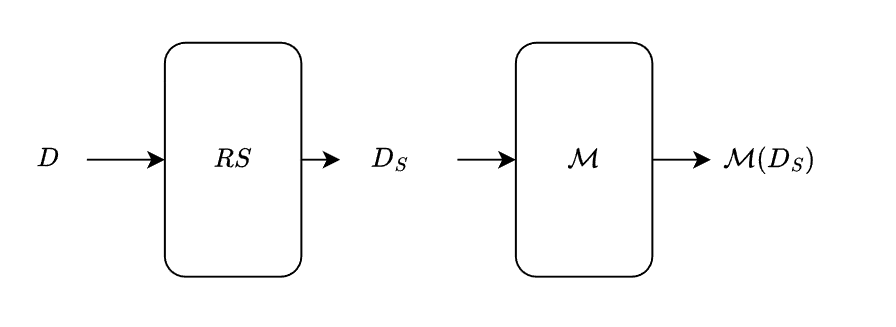
\includegraphics[width=0.8\textwidth]{assets/1.png}
    \caption{The First Method}
\end{figure}
\begin{figure}[ht]
    \centering
    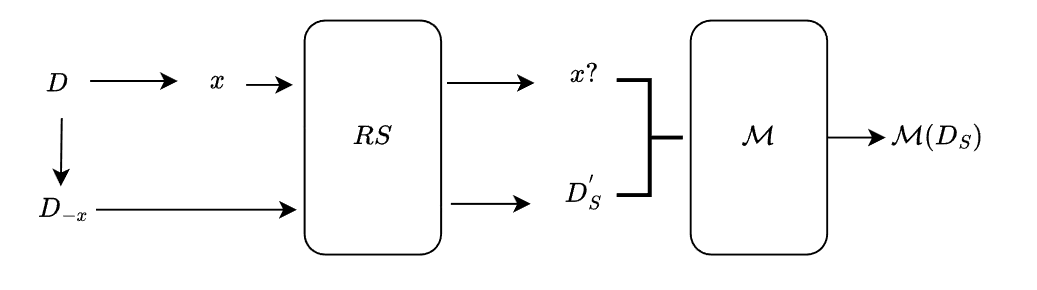
\includegraphics[width=0.8\textwidth]{assets/2.png}
    \caption{The Second Method}
\end{figure}
\newpage
\paragraph{First method}
consider all $D_S$ that make $\mathcal{M}_{t}^{f}(D_S) \in S$ and utilize \textbf{Law of total probability}, we can get as follows:
\begin{equation}
    Pr(S_f(D, \epsilon, t) \in S) = \sum_{D_S \subset D}Pr(RS(D, \epsilon, t) = D_S) \cdot Pr(\mathcal{M}_{t}^{f}(D_S) \in S)
\end{equation}

Apply the same reasoning to $D_{-x}$, we can get as follows:
\begin{equation}
    Pr(S_f(D_{-x}, \epsilon, t) \in S) = \sum_{D_{S}^{'} \subset D_{-x}}Pr(RS(D, \epsilon, t) = D_{S}^{'}) \cdot Pr(\mathcal{M}_{t}^{f}(D_{S}^{'}) \in S)
\end{equation}

\paragraph{Second method}
We can also represents $Pr(S_f(D, \epsilon, t) \in S)$ as follows:
\begin{equation}
    \begin{aligned}
        Pr(S_f(D, \epsilon, t) \in S) & = (1 - \pi_x)\sum_{D_{S}^{'} \subset D_{-x}}Pr(RS(D_{-x}, \epsilon, t) = D_S^{'}) \cdot Pr(\mathcal{M}_{t}^{f}(D_{S}^{'}) \in S)      \\
                                      & \quad + \pi_x\sum_{D_{S}^{'} \subset D_{-x}}Pr(RS(D_{-x}, \epsilon, t) = D_{S}^{'}) \cdot Pr(\mathcal{M}_{t}^{f}(D_{S+ x}^{'}) \in S) \\
    \end{aligned}
\end{equation}

Since $M_{f}^{t}$ is $t$-differentially private, for neighbor datasets $D_S^{'}$ and $D_{S + x}^{'}$, we can get as follows:
\begin{equation}
    \begin{aligned}
        Pr(\mathcal{M}_{t}^{f}(D_{S + x}) \in S) & \leq e^{t} Pr(\mathcal{M}_{t}^{f}(D_S) \in S) \\
    \end{aligned}
\end{equation}

Substitute into the above equation, we can get as follows:
\begin{equation}
    \begin{aligned}
        Pr(S_f(D, \epsilon, t) \in S) & = (1 - \pi_x)\sum_{D_{S}^{'} \subset D_{-x}}Pr(RS(D_{-x}, \epsilon, t) = D_{S}^{'}) \cdot Pr(\mathcal{M}_{t}^{f}(D_{S}^{'}) \in S)     \\
                                      & \quad + \pi_x\sum_{D_{S}^{'} \subset D_{-x}}Pr(RS(D_{-x}, \epsilon, t) = D_{S}^{'}) \cdot Pr(\mathcal{M}_{t}^{f}(D_{S+ x}^{'}) \in S)  \\
                                      & \leq (1 - \pi_x)\sum_{D_{S}^{'} \subset D_{-x}}Pr(RS(D_{-x}, \epsilon, t) = D_{S}^{'}) \cdot Pr(\mathcal{M}_{t}^{f}(D_{S}^{'}) \in S)     \\
                                      & \quad + \pi_x e^{t}\sum_{D_{S}^{'} \subset D_{-x}}Pr(RS(D_{-x}, \epsilon, t) = D_{S}^{'}) \cdot Pr(\mathcal{M}_{t}^{f}(D_S^{'}) \in S) \\
                                      & = (1 - \pi_x + \pi_x e^{t}) Pr(S_f(D_{-x}, \epsilon, t) \in S)
    \end{aligned}
\end{equation}

Consider the value of $\pi_x$:
\begin{itemize}
    \item If $\epsilon_x \geq t$, then $\pi_x = 1$, $1 - \pi_x + \pi_x e^{t} = e^{t} \leq e^{\epsilon_x}$.
    \item If $\epsilon_x < t$, then $\pi_x = \frac{e^{\epsilon_x} - 1}{e^t - 1}$, $1 - \pi_x + \pi_x e^{t} = e^{\epsilon_x}$.
\end{itemize}
In conclusion, we can get:
\begin{equation}
    Pr(S_f(D, \epsilon, t) \in S) \leq e^{\epsilon_x} Pr(S_f(D_{-x}, \epsilon, t) \in S)
\end{equation}

So the sample mechanism with any $t > 0$ and any $i \in [n]$ is $\{\epsilon_i\}_{i\in [n]}$-PDP.

\end{document}